\documentclass{cumcm}


% \title{text}这里是显示在第三页的文章标题
\title{机场的出租车问题}
% \displaytitle{text} 这里是显示在承诺书上的文章标题,注意,不能换行,如果题目特别长,要进行适当的缩写
\displaytitle{机场的出租车问题}
% \school{text}命令用于在承诺书上显示学校名称。按要求,此处应填写全称
\school{上海交通大学}
% 以下命令分别显示队员、指导教师姓名以及队伍编号
\authorone{刘畅}
\authortwo{谢哲}
\authorthree{胡胜超}
\advisor{}
\teamnumber{未知报名号}
\dateyear{2019}
\datemonth{9}
\dateday{7}

\begin{document}

% 这里用于打印承诺书以及编号页
 
%\newpage
\thispagestyle{empty} %取消当前页码
{\Large \heiti \begin{center}\the\year~高教社杯全国大学生数学建模竞赛\par\vspace{0.5\ccwd}\par
{\ziju{1}承诺书}\end{center}\par\vspace{1\ccwd}\par}
\renewcommand{\baselinestretch}{1.5}\normalsize
{\zihao{-4}%
我们仔细阅读了中国大学生数学建模竞赛的竞赛规则。\par
我们完全明白,在竞赛开始后参赛队员不能以任何方式(包括电话、电子邮件、网上咨询等)
与队外的任何人(包括指导教师)研究、讨论与赛题有关的问题。\par
我们知道,抄袭别人的成果是违反竞赛规则的, 如果引用别人的成果或其他公开的资料
(包括网上查到的资料),必须按照规定的参考文献的表述方式在正文引用处和参考文献中明确列出。\par
我们郑重承诺,严格遵守竞赛规则,以保证竞赛的公正、公平性。如有违反竞赛规则的行为,我们将受到严肃处理。\par
\par\vspace{2\ccwd}\par
\raisebox{1ex}[0pt]{我们参赛的题目是:}\vbox{\hbox to11.4cm{\hfil \the\displaytitle \hfil}
        \protect\vspace{0.6truemm}\relax
        \hrule depth0pt height0.15truemm width11.4cm}\par
\vspace{1mm}
\raisebox{1ex}[0pt]{我们的参赛报名号为(如果赛区设置报名号的话):}\vbox{\hbox to5.75cm{\hfil \the \teamnumber  \hfil}
        \protect\vspace{0.6truemm}\relax
        \hrule depth0pt height0.15truemm width5.75cm}\par
\vspace{1mm}
\raisebox{1ex}[0pt]{所属学校(请填写完整的全名):}\vbox{\hbox to9.12cm{\hfill \the\school \hfill}
        \protect\vspace{0.6truemm}\relax
        \hrule depth0pt height0.15truemm width9.12cm}\par
\begin{tabular}{lcp{8.82cm}c}
\hspace{-2.1mm}\raisebox{-1mm}[0pt]{参赛队员(打印并签名): }&\raisebox{-1mm}[0pt]{1、}& \raisebox{-1mm}[0pt]{\the\authorone\hfill{}}& \\ \cline{3-3}
   &\raisebox{-1mm}[0pt]{2、}& \raisebox{-1mm}[0pt]{\the\authortwo\hfill{}}& \\ \cline{3-3}
   &\raisebox{-1mm}[0pt]{3、}& \raisebox{-1mm}[0pt]{\the\authorthree\hfill{}}& \\ \cline{3-3}
\end{tabular}
\par
\vspace{10mm}
\raisebox{1ex}[0pt]{指导教师或指导教师组负责人(打印并签名):}\vbox{\hbox to6.65cm{\the\advisor \hfil}
        \protect\vspace{0.6truemm}\relax
        \hrule depth0pt height0.15truemm width6.65cm}\par
\vspace{5mm}
{}\hspace{10cm}日期:\uline{\hspace{0.5em}\the\dateyear\hspace{0.5em}}年\uline{\hspace{0.5em}\the\datemonth\hspace{0.5em}}月 
\uline{\hspace{0.5em}\the\dateday\hspace{0.5em}}  日
\par
\vspace{2cm}
\hrulefill\par\vspace{2\ccwd}\par
赛区评阅编号(由赛区组委会评阅前进行编号):
}
\renewcommand{\baselinestretch}{1.3}\normalsize
\newpage
\thispagestyle{empty} %取消当前页码
{\Large \heiti \begin{center}\the\year~高教社杯全国大学生数学建模竞赛\par\vspace{0.5\ccwd}\par
{\ziju{1}编号专用页}\end{center}\par\vspace{1\ccwd}\par}
{\zihao{-4}%
\par\vfill
赛区评阅编号(由赛区组委会评阅前进行编号):\par\vfill\vfill

赛区评阅记录(可供赛区评阅时使用):\vspace{1\ccwd}

\begin{center}
\resizebox{.9\textwidth}{!}{
\begin{tabular}{|c|*{10}{p{.09\textwidth}|}}
\hline
\makecell{评\\阅\\人}&&&&&&&&&&\\
\hline
\makecell{评\\分}&&&&&&&&&&\\
\hline
\makecell{备\\注}&&&&&&&&&&\\
\hline
\end{tabular}
}
\end{center}\vspace{1\ccwd}

全国统一编号(由赛区组委会送交全国前编号):\par\vfill\vfill

全国评阅编号(由全国组委会评阅前进行编号):\par\vfill\vfill\vfill
}
\renewcommand{\baselinestretch}{1.3}\normalsize

\newpage

\begin{minipage}{0.9\textwidth}
\centering\LARGE\textbf{出租车的动态调度问题}
\end{minipage}

% 摘要和关键字
\begin{abstract}
	在大数据时代,通过分析一些重要的客流量大的枢纽场所的客流数据,设计出交通枢纽的合理的调度方式,成为了一个非常重要的课题。本题以机场陆侧的出租车交通组织模式为切入点,站在不同的角度对机场出租车的组织模式提出了需求。本文使用了基于排队论构建的模型,分析了不同场景下,不同的出租车组织模式对出租车运输效率的影响。利用MATLAB进行了交通场景的仿真模拟,并使用多种优化算法求解出最优解,最后分析了模型的依赖性和优缺点。\par
	\textbf{针对问题一}\quad
	在问题一中,由于出租车司机能观测到某时间段抵达的航班数量和“蓄车池”里已有的车辆数,故针对选择排队等待拉客还是直接选择返回市区应以这能观测到的两个参数作为主要参考依据。因此,我们只需要简单地做出线性规划问题,求出对应于不同参数采取不同的选择。由于航班来临的时刻人数会出现一种符合正态分布的曲线到达‘乘车区’,而此时‘蓄车池’中出租车数量的多少又会正比于等待时间,于是可以推测出选择等待后需要等待的时间,然后假定在相同长一段时间内,直接返回市区考虑平均每分钟的收益和在等待区载客并载客后的收益进行比较来综合判断如何选择。\par
	\textbf{针对问题二}\quad
	根据河南郑州新郑国际机场的出租车动态变化网页,经过一昼夜爬虫后得到一昼夜的出租车的动态变化表,根据该段时间内到达郑州航班的多少,选择以2个小时内作为基准,代入问题一所建立的出租车等待模型,综合对比理论值和实际值之间的区别并求取平均值,求得平均相对误差不超过0.1036.然后根据问题一得到的分界值来进行选择。在机场出租车系统正常调度的情况下,相对误差不超过0.1,但同时也对当时出租车以外的交通系统的变化有着较大的依赖性。\par
	\textbf{针对问题三}\quad
	对于题目给定的双车道并行的场景,设计了不同的“上车点”和乘客安排方式。对于单停车道模型和双停车道模型,本文分别使用了排队论中的$M/M/1$和$M/M/2$模型对乘客在队列中的平均等待时间进行了分析和计算。本文对两种不同的排队模型进行了比较,得出了在不同条件下优先采取某种排队模型的结论。并证明了在乘客到达速率小于出租车到达速率的条件下,优先采用双停车道模型,在乘客到达速率大于出租车到达速率的条件下,优先考虑单停车道模型。\par
	\textbf{针对问题四}\quad
	对于问题四,我们认为载客的行程越长,出租车的载客收益也就越大,于是采取对载客行程较短的出租车给予他们一定的优先权。综合考虑出租车在上一次等待时长和这一次载客的收益,得出该出租车的“优先值”,然后设置一个“优先阙值”,大于该“优先阙值”即可直接插入到优先级高的车道,并且拥有优先载客的权利,但是对于低优先级的车,被插队次数不应超过一定的值,于是通过对上述优先值算法,“优先阙值”,被插队次数最大值进行遗传算法,退火算法,粒子群算法得到每个出租车收益的方差的最小值时所满足的条件,根据该条件来安排一个可行的“优先”方案。
\\\par
\textbf{关键词\quad 排队论\quad 动态调度\quad 遗传算法\quad 退火算法\quad 粒子群算法}
\end{abstract}

\newpage
\section{问题重述}
\subsection{问题背景}
出租车是乘客往返市区与机场的主要交通方式之一。机场有客流密度大的特点,而乘客需要在固定的出租车上客点乘车。由于上客点地点和条件有限,且上客的效率受到了乘客、机场航班、出租车司机等多种因素的影响。所以需要一种优化的解决方案能够提高乘客在出租车上客点的乘车效率,以减少乘客和出租车司机的等待时间。\par
对于司机而言,离开下客区后,选择直接离开机场空载返回、或是排队等待载客,将会对司机的收益产生影响,而排队的等待时间便是影响司机收益的关键。所以,需要一种可靠的算法,能够根据便于获得的一些数据来协助司机的决策过程。此外,由于出租车乘车乘客前往目的地的随机性,部分司机可能在等待较长时间之后,乘客前往的目的地较近,从而导致司机的收益相对偏低。所以需要一种合理的方式,使得出租车司机的收入能够保持尽可能均衡。
\subsection{问题重述}
国内机场一般将出租车乘车区分为上客区和下客区两个分开的区域,并且对于离开上客区的出租车,司机可以根据的意愿选择放空车辆直接离开或前往“蓄车池”载客。对于司机,他们可以得到当前“蓄车池”内的车的数量以及当前的航班数量来决定是否进入“蓄车池”等待,并且司机通常还可以根据自己的经验,结合季节、时间等因素判断乘客数量的多少。如果司机选择直接放空返回,则可能会有返回时的空载费用和载客的潜在收益的损失。对于机场管理者,他们需要在上客地点的等候区采取“分批定量”放行的措施来让乘客依次进入上客区乘车。\par
\begin{figure}[H]
	\centering
	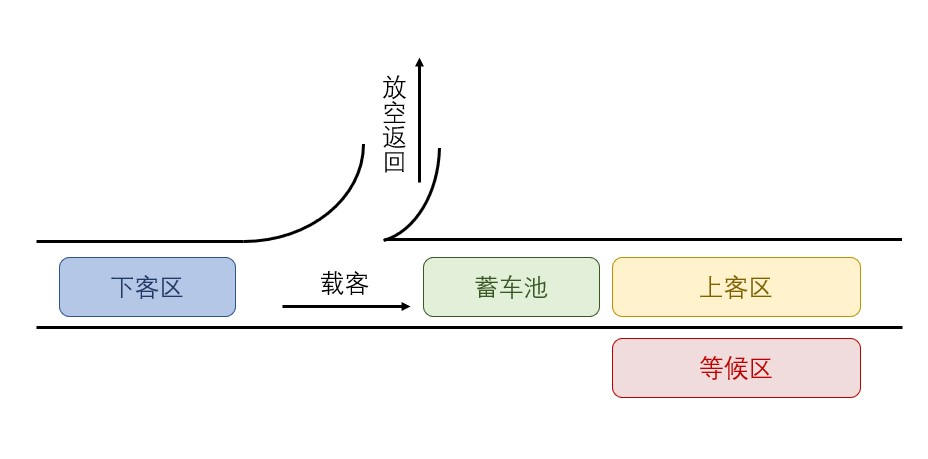
\includegraphics[width=1.0\textwidth]{img/taxi_example.jpg}
	\caption{机场出租车乘车区域示意图}
	\label{taxi_example}
\end{figure}
\newpage
根据以上条件,我们需要研究如下的4个问题:
\begin{enumerate}[(1)]
	\item 建立一个模型,用于计算得到出租车司机载客与放空返回的选择策略。建立模型时综合考虑机场在不同时间的旅客数量的变化规律和其它的相关因素,使得出租车的做出的策略能够使其收益最大化。
	\item 获取国内某一机场的实际数据,根据建立的模型和机场的实际数据计算出司机的决策策略,将计算得到的数据(如预期出租车等待时间)与真实数据进行比较和分析,并由此可以出模型的合理性与对相关因素的依赖程度。
	\item 机场在高峰时段,乘客和出租车可能会排起长队。机场乘车区设置有两条并行车道,建立一个模型,确定合理的“上车点”的位置,并合理安排出租车的行驶方式和乘客的上车方式,在确保安全的前提下,使得乘客的平均排队时间能够最短,乘车效率达到最大。
	\item 出租车在机场载客的目的地是随机的,并且出租车司机无法自主选择载客或拒绝载客,所以出租车司机的收益可能会出现不均衡的情况。为了解决这个问题,考虑给予返回的短途载客的司机在下一次载客时的优先权。建立一个模型,给出可行的优化方案,使得出租车司机们的收益能够尽可能均衡。
\end{enumerate}

\section{模型假设}
\begin{enumerate}
	\item 考虑到每个人上车的时间相差较小,可以认为每个人从乘车区上车到出租车起步离开的时间固定,我们记这个时间为$t_0$。
	\item 由于到港航班的分布与相对均匀,本文认为在考虑的一段时间之内,航班到达机场的时间是等间隔的。
	\item 根据统计学规律,在一段时间之内,各个航班到达的乘客前往出租车乘车区域乘车的人数符合泊松分布。
	\item 根据统计学规律,每一个到达航班的需要乘坐出租车的乘客到达出租车乘车等候区的时间满足正态分布。
	\item 由于汽车在等待时由于仍在运行中,其耗油量近似为正常运行时的$\frac{1}{2}$,所以可以认为出租车在“蓄车池”等待期间消耗的油量较正常运行时更低。
	\item 根据统计学规律,从机场离开的出租车前往目的地的距离满足正态分布的规律。
\end{enumerate}

% 符号变量设置
\newcommand{\flightnum}{$N_f$}
\newcommand{\taxinum}{$N_c$}
\newcommand{\waittime}{$t_w$}

\section{符号说明}
表\ref{table-symbol}列出了本文需要的符号。
\begin{table}[H]
	\centering
	\caption{符号说明} 
	\label{table-symbol}
	\begin{tabular*}{0.65\textwidth}{ccc}
		\toprule
		符号 & 意义 & 单位 \\
		\midrule
		\flightnum & 一段时间内的航班数量 & 架 \\
		\taxinum & 蓄车池内的出租车数量 & 辆 \\
		$T$ & 模型考察的总时间长度 & $min$ \\
		\waittime & 出租车司机等待的时间 & $min$ \\
		$t_r$ & 出租车从机场返回市区的时间 & $min$ \\
		$n_i$ & 第$i$架航班上需要乘坐出租车的人数 & 人 \\
		$M_0$ & 一架航班乘坐出租车的人数最大值 & 人 \\
		$\Delta t_f$ & 航班的时间间隔 & $min$ \\
		$p_i$ & 第$i$架航班乘客乘坐出租车的概率 & \\
		$q_i$ & 第$i$架航班乘客抵达候车区的时间分布 & \\
		$\lambda_1$ & 航班乘坐出租车人数分布的均值 & \\
		$\lambda_2$ & 乘客到达乘车区时间分布参数 & \\
		$\mu_1$ & 乘客到达乘车区时间正态分布均值 & \\
		$\mu_2$ & 乘客上车间隔指数分布参数 & \\
		$N$ & 开始时蓄车池内出租车能够容纳的乘客人数 & 人 \\
		$\overline{t_0}$ & 平均每辆车上车所需耗费时间 & $min$ \\
		$t_1$ & 到达等候区乘客累计达到$N$的时刻 & $min$ \\
		$t_2$ & 载客出租车返回市区的时刻 & $min$ \\
		$t_{extra}$ & 出租车额外等待的时间 & $min$ \\
		$\varepsilon_0$ & 平均每辆车的载客数 & 人$/$辆 \\
		$E_1$ & 每辆出租车从空载返回到$t_2$时刻的利润 & 元 \\
		$E_2$ & 每辆出租车从进入蓄车池到$t_2$时刻的利润 & 元 \\
		$\overline{E_o}$ & 出租车正常行驶平均每分钟油费 & 元$/min$ \\
		$\overline{E_{wo}}$ & 出租车排队时平均每分钟油费 & 元$/min$ \\		$\overline{E_i}$ & 出租车在市区内运营平均收入 & 元$/min$ \\
		$\overline{E_c}$ & 出租车平均载客返回收入 & 元 \\
		$W_{q1}$ & 双车道停车模型乘客平均等待时间 & $min$ \\
		$W_{q2}$ & 单车道停车模型乘客平均等待时间 & $min$ \\  
		$C$ & 单车道停车模型服务台数目 & \\
		$\overline{E_a}$ & 机场出租车单位时间平均收入 & 元$/min$ \\
		$d$ & 行驶里程 & $m$ \\
		$\omega$ & 出租车返程收入 & 元 \\
		\bottomrule
	\end{tabular*}
\end{table}

\section{问题分析}
\subsection{问题一的分析}
问题一的本质就是要建立一个出租车司机关于一段时间内航班数量\flightnum 与当前蓄车池内出租车的数量\taxinum 的决策模型$f\left(\mbox{\flightnum},\mbox{\taxinum}\right)$,而这个模型可以分成如下的两个部分:
\begin{enumerate}[(1)]
	\item 出租车时间等待时间$t$与航班数量\flightnum 和蓄车池内出租车数量\taxinum 的预测模型$\mbox{\waittime}\left(\mbox{\flightnum},\mbox{\taxinum}\right)$,通过计算机模拟的方法,得出可行域内的不同\flightnum 和\taxinum 下的\waittime 的数值,可以绘制出\waittime 关于\flightnum 和\taxinum 的函数关系图像。
	\item 建立数学模型,得到出租车不载客利润$E_1$和出租车载客利润$E_2$与出租车等待时间\waittime 之间的函数关系$E_1(\mbox{\waittime})$和$E_2(\mbox{\waittime})$,并做出出租车司机的决策$\max(E_1(\mbox{\waittime}),E_2(\mbox{\waittime}))$,由此得到出租车司机关于等待时间的决策函数$E(\mbox{\waittime})$。
\end{enumerate}
\par
将如上的两个数学模型得到的函数$t\left(\mbox{\flightnum},\mbox{\taxinum}\right)$和$E(\mbox{\waittime})$联立,最终得到出租车司机关于\flightnum 和\taxinum 的决策函数$f(\mbox{\flightnum},\mbox{\taxinum})$。

\subsection{问题二的分析}
问题二的本质是需要根据搜集国内的某一个机场的实际数据,带入问题一中得到的模型,得到不同条件下出租车司机的最佳选择策略,由此对问题一中的模型进行数值上的验证,所以问题二的解决需要分为如下几个步骤:
\begin{enumerate}[(1)]
	\item 收集国内某一城市的机场航班数量分布情况、出租车出入场、场内出租车数量、该城市机场到市区出租车均价、单位时间油耗价格和出租车单位时间正常收入。
	\item 根据收集到的数据,带入问题一中建立的模型,计算出租车司机等待时间的阈值$t_{w0}$。
	\item 根据收集到的参数,绘制出$t_w-N_f,N_c$图像,作平面$\alpha:t_w=t_{w0}$,得到平面$\alpha$和$t_w$平面的交线$l:\alpha\cap t_w(N_f,N_c)$,则$l$即为$t_w$的阈值曲线。
	\item 根据收集到的数据,随机抽取部分数据,带入上述模型进行计算,得到预计的等待时间$\hat{t_w}$,与实际的等待时间进行比较,分析模型的误差和对相关因素的敏感程度。
\end{enumerate}

\subsection{问题三的分析}
问题三要求给出一个合理的乘客“上车点”设置方式,在保证安全的前提之下,能够降低乘客的平均等待时间。在此前提之下,可以建立如下的两种数学模型:
\begin{enumerate}[(1)]
	\item \textbf{双车道停车模型。}两条并行车道都可以停车、上车,但为安全考虑,只在最前端开设一个上车点供上车,乘客可以从出租车队列的最前端穿越马路乘坐出租车。这种模型,可以用排队论中的$M/M/2$模型表示,并通过排队论模型计算出乘客的平均等待时间$W_{q1}$。
	\item \textbf{单车道停车模型。}两条并行车道,靠航站楼的一边可以设置多个停车点,排多条队伍上客,另一条车道用于出租车车辆通行,使得每个停车点出租车相互不干扰。这种模型,可以用排队论中多个独立的$M/M/1$模型表示,并可以由此用排队论模型计算出乘客的平均等待时间$W_{q2}$。
\end{enumerate}
\par
通过对如上的两种数学模型进行分别建模和求解,可以分别求解出两种模型中的乘客平均等待时间$W_q$,并根据平均等待时间对其进行比较,从而得到两种方案中的最优方案。
\subsection{问题四的分析}
问题四的题目描述了一个机场出租车目的地的随机分布导致的收益不均衡的问题,并要求给出优化方案。而对于机场而言,可行的优化方案是设定一个最优的用于对出租车进行分类的“优先级”计算方式。并设置一个合理的阈值,来划分“高优先级”和“低优先级”,并允许“高优先级”的出租车能够在下一次返回机场时,通过“插队”的方式优先载客,缩短等待时间。对于这个问题,我们可以先使用计算机模拟出租车系统的运行过程,计算出每辆出租车的单位时间的平均收益,由此计算出所有出租车的收入的方差。之后可以使用遗传算法等多种算法来优化模型中的各种参数,得到最合理的优先级计算方法和高低优先级划分阈值。
\par
可以将这个问题分为以下几个过程来解决:
\begin{enumerate}[(1)]
	\item 建立数学模型,给出出租车优先级关于各个自变量与参数的关系。
	\item 编写计算机程序,模拟机场和出租车的运行过程,并且根据初始设定的参数计算出租车的优先级,最终统计出出租车单位时间内收益的方差。
	\item 使用优化算法,找到使方差值最小的参数值,并完成模型的灵敏度分析和评价。
\end{enumerate}
\section{模型建立}
针对本题,本文一共建立了三个数学模型:用于出租车司机决策的模型、用于设置机场停车点的模型、用于短途载客返回出租车优先权的模型。下面依次对这三个模型的建立作详细说明。
\subsection{用于出租车司机决策的模型}
用于出租车司机决策的模型一共分为出租车等待时间$\mbox{\waittime}\left(\mbox{\flightnum},\mbox{\taxinum}\right)$和出租车司机决策$E(\mbox{\waittime})$两个部分,以下依次描述这两个模型的具体建立过程,并将两个模型综合得到最终的决策模型。
\subsubsection{出租车等待时间}
乘客在乘车区排队等待出租车采用排队论中$M/G/1/\infty/N/FCFS$模型进行分析。出租车的等待时间分为两部分,一部分是乘客上车占用的时间$Bt_0$,另一部分是由于乘坐出租车的乘客前往乘车点的时间间隔过大,导致的出租车空闲等待的时间:
\begin{equation}
	t_{extra}=\sum_it_{extrai}
	\label{eq:textrafunc}
\end{equation}
由此可以得到等待时间\waittime 的计算公式:
\begin{equation}
	\mbox{\waittime}=\mbox{\taxinum}\overline{t_0}+t_{extra}
	\label{eq:tfunc}
\end{equation}
\par
航班的之间的间隔$\Delta t_f$与总时间$T$和航班数目\flightnum 满足如下的关系:
\begin{equation}
	\Delta t_f=T/\mbox{\flightnum}
	\label{eq:deltatf}
\end{equation}
对于一段时间内航班到达的数量分布,本文认为其满足均匀分布的规律。其中,对于每一架航班乘坐出租车的人数$n_i$,其与每一架航班乘坐出租车的最大人数$M_0$和该架航班上的乘客乘车概率$p_i$满足如下关系:
\begin{equation}
	n_i=M_0·p_i
	\label{eq:passengernum}
\end{equation}
由此,我们可以通过公式\ref{eq:passengernum}来确定不同时间段到达机场的乘客的数量,对于概率$p_i$,本文认为其满足均值为$\lambda_1$的泊松分布:
\begin{equation}
	p_i(X=k)=\frac{\lambda_1}{k!}e^{-\lambda_1}
	\label{eq:pi}
\end{equation}
对于进入等候区排队的乘客,我们使用FCFS模型。其中对于每一架到达的航班,从航班到达,至需要乘坐出租车的乘客抵达出租车等候区排队的时间,本文认为其关于时间的分布满足均值为$\mu_1$,标准差为$\sigma$的正态分布:
\begin{equation}
	q_i((i-1)\Delta t_f+t)=\frac{1}{\sqrt{2\pi}\sigma}e^{-\frac{(t-\mu_1)^2}{2\sigma^2}},\quad t\ge0
	\label{eq:qi}
\end{equation}
对于此时在蓄车池中的车辆数量,其数量\taxinum 与能够承载的乘客人数$N$满足如下关系:
\begin{equation}
	N=\mbox{\taxinum}·\varepsilon_0
	\label{eq:N}
\end{equation}
根据以上描述的符号关系,与式\ref{eq:N}联立,我们可以列出承载乘客与到达乘客的关系:
\begin{equation}
	\sum_i\int_0^{t_1}M_0\cdot p_iq_i(t)\mathrm{d}t=\mbox{\taxinum}\cdot\varepsilon_0
\end{equation}
\subsubsection{出租车收益与等待时间关系}
出租车的收益可以分为空再返回和等待载客两部分进行分别分析。分析的时间段为出租车下客完成(时间起点),至载客返回的出租车抵达市区的时间$t_2$。
\begin{enumerate}[(1)]
	\item \textbf{空载返回出租车收益。}\par
	空载返回的出租车由于无需等待,所以其能够在空载返回市区后直接载客运营,故空载返回的出租车的收入为其在市区运营时的收入,其耗费为全程的油费。于是我们可以得到如下空载返回出租车收益$E_1$关于$t_2$的关系:
	\begin{equation}
		E_1(t_2)=\overline{E_i}\cdot(t_2-t_r)-\overline{E_o}\cdot t_2
		\label{eq:E1}
	\end{equation}
	\item \textbf{载客出租车收益。}\par
	由于载客出租车需要在蓄车池内等待乘客,而根据假设,蓄车池内等待不消耗任何成本,所以载客出租车的收入为载客从机场返回市区的收入,消耗为返回市区时的油耗。于是我们可以得到如下空载返回出租车的收益$E_2$的表达式:
	\begin{equation}
		E_2=\overline{E_c}-t_r\cdot\overline{E_o}-t_2\cdot\overline{E_{wo}}
		\label{eq:E2}
	\end{equation}
\end{enumerate}
\par
此外,我们还可以得到出租车等待时间\waittime 和载客出租车返回市区的时间$t_2$时间的关系:
\begin{equation}
	t_2=\mbox{\waittime}+t_r
	\label{eq:t2}
\end{equation}
将式\ref{eq:E1}、\ref{eq:E2}、\ref{eq:t2}联立,我们可以得到用于司机决策的\waittime 的阈值,由此建立用于出租车司机决策的模型。
\subsection{用于设置机场停车点的模型}
用于设置机场停车点的模型一共分为两类:双车道停车模型和单车道停车模型。先分别建立两种模型。
\begin{enumerate}[(1)]
	\item \textbf{双车道停车模型。}\par
	\begin{figure}[H]
		\centering
		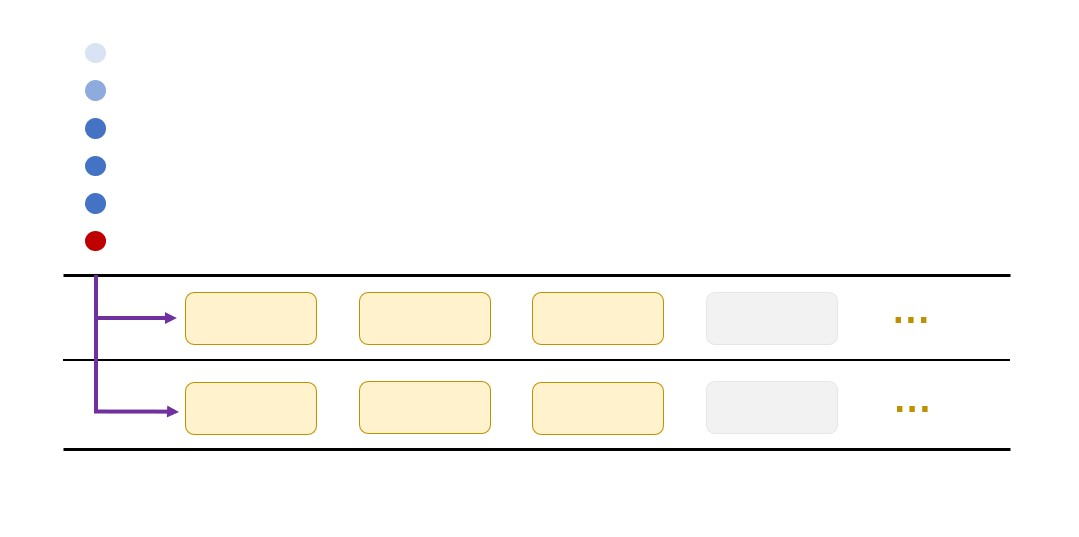
\includegraphics[width=0.9\textwidth]{img/problem3_double.jpg}
		\caption{双车道停车模型示意图}
		\label{fi:problem3double}
	\end{figure}
	双车道停车模型示意图如图\ref{fi:problem3double}所示。为了安全考虑,由于在这种模型中,乘客需要穿越马路到达外侧车道乘车,所以乘客不应当在汽车可能行驶的队列中后部穿越马路乘车,模型中的“上车点”只有一个,设置在出租车队列的最前方。队列中的候车乘客可以等待车辆停稳之后,从出租车队列的最前方穿越马路,在两辆车中选择一辆出租车搭乘。\par
	在上述前提条件下,采用经典的排队论建立模型。这是一个典型的单队列、双服务台模型,并且顾客到达时间满足参数为$\lambda_2$的负指数分布,服务时间(即相邻前后辆车在队列最前方停稳的时间间隔)满足参数为$\mu_2$的负指数分布,即排队论中的$M/M/2$模型。根据该排队论模型,我们有如下公式\cite{queuebook}:
	\begin{equation}
		W_{q1}=\frac{\lambda_2}{\mu_2(\mu_2-\lambda_2)}
		\label{eq:wq1}
	\end{equation}
	根据式\ref{eq:wq1}即可计算顾客的平均等待时间,从而对双车道停车模型的乘车效率进行评估,并与单车道停车模型进行比较,得到较优的方案。
	\item \textbf{单车道停车模型。}\par
	\begin{figure}[H]
		\centering
		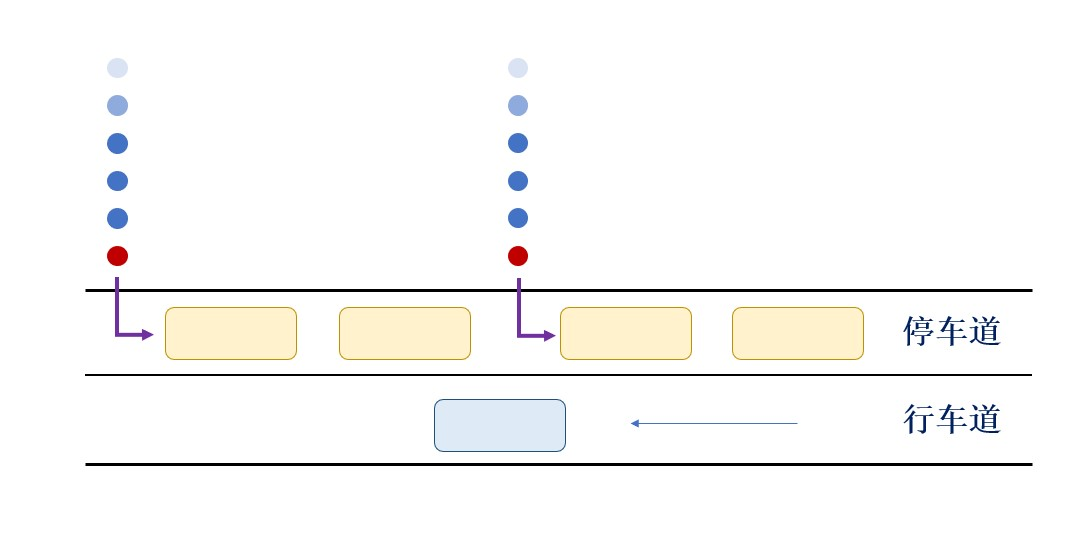
\includegraphics[width=0.9\textwidth]{img/problem3_single.jpg}
		\caption{单车道停车模型示意图}
		\label{fi:problem3single}
	\end{figure}
	单车道停车模型示意图如图\ref{fi:problem3single}所示。在这种模型中,靠近航站楼的一侧可以设置多条队伍,对应多个停车点。在排队论中,这个模型即为多条互相独立的队伍和多个服务台,本文定义服务台的数量为$C$。在这个模型中,顾客到达的时间间隔符合参数为$\frac{\lambda_2}{C}$的负指数分布,车辆服务时间符合参数为$\frac{\mu_2}{C}$的负指数分布。所以该模型为$C$个互相独立的$M/M/1$模型的组合。设变量$\rho$满足:
	\begin{equation}
		\rho=\frac{\frac{\lambda_2}{C}}{C\cdot\frac{\mu_2}{C}}=\frac{\lambda_2}{C\mu_2}
		\label{eq:rho}
	\end{equation}
	可以用如下的公式\cite{queuebook}计算其顾客平均等待时间$W_{q2}$:
	\begin{equation}
		W_{q2}=\frac{1}{\lambda_2}\cdot\frac{C^C\rho^{C+1}\left(\sum\limits_{n=0}^{C-1}\frac{C^n}{n!}\rho^n+\frac{C^C}{C!}\cdot\frac{\rho^C}{1-\rho}\right)^{-1}}{C!\left(1-\rho\right)^2}
		\label{eq:wq2}
	\end{equation}
\end{enumerate}
分别带入实际数据,计算式\ref{eq:wq1}和式\ref{eq:wq2}的值,将二者进行比较,可以得出相应的最优解。
\subsection{用于短途载客返回出租车优先权的模型}
对于该模型,假设出租车从机场出发,抵达目的地的里程满足均值为$\mu$,标准差为$\sigma$的正态分布$d\sim N(\mu,\sigma^2)$,并有如下关于里程阈值$d_0$的返回策略:
\begin{equation}
	\mbox{返回策略}
	\begin{cases}
		\mbox{  远程,不返回机场}\quad & t\ge t_0 \\
		\mbox{  近程,50\%几率返回机场}\quad & t<t_0
	\end{cases}
\end{equation}
定义优先级函数$r(\overline{E_a},t_w)$满足:
\begin{equation}
	r(\overline{E_a},t_w)=\alpha\cdot\overline{E_a}-t_w
	\label{eq:r}
\end{equation}
其中$\alpha$为参数。
\par
定义单位时间平均收益$\overline{E_a}$满足:
\begin{equation}
	\overline{E_a}=\frac{\omega(d)-\overline{E_o}\cdot t_{\mbox{运行}}}{t_w+t_{\mbox{运行}}}
	\label{eq:ea}
\end{equation}
其中$\omega(d)$为出租车的收费,与路程$d$相关,可以代入某城市的出租车具体收费价格进行价格计算。\par
定义优先级阈值$r_0$,规定满足如下关系:
\begin{equation}
	\mbox{优先级别}
	\begin{cases}
		\mbox{低级}\quad & r(\overline{E_a},t_w)>r_0 \\
		\mbox{高级}\quad & r(\overline{E_a},t_w)\le r_0 \\
	\end{cases}
\end{equation}
\par
机场的出租车入口分为两条车道,分别为普通车道和优先车道。当出租车第一次进入机场时,认为其默认进入普通车道排队;当出租车在短时间内再次返回机场并选择载客时,机场会根据前述规则判断该出租车辆的优先级,优先级高的车辆进入优先车道排队,优先级低的车辆进入普通车道。优先车道与普通车道按照$\beta:1$的比例进入上车区载客。每次车辆进入机场时,上一次进入机场的数据即被清空,其相关数据将被重新计算。\par
定义评价函数为出租车单位时间平均收入的方差:
\begin{equation}
	\sigma^2(\overline{E_a})=\frac{1}{N_m}\sum_i(\overline{E_{ai}}-\mu_m)^2
\end{equation}
其中$N_m$代表总出租车数目,$\mu_m$代表出租车的总平均单位时间收益。该模型本质是一个多参数的最优化问题,目标是:$\min\quad\sigma^2(\overline{E_a})$。使用优化算法得到最优解及其参数,即完成此题的目标。

\section{问题解答}
\subsection{问题一的解答}
对于问题一,本文建立了出租车司机的决策模型。这个模型分为出租车等候时间和出租车收益两个部分,根据以上建立的模型分别对这两个模块进行求解。\par
对于出租车等候时间,在选定的时间范围之内,建立了航班到达、乘客前往乘车区,和乘客在乘车区排队上车的模型,即出租车的等待时间\waittime 关于航班数量\flightnum 和蓄车池内出租车数量\taxinum 的函数关系,并使用如图\ref{fi:program1}所示的程序模拟了这一过程。
\begin{figure}[H]
	\centering
	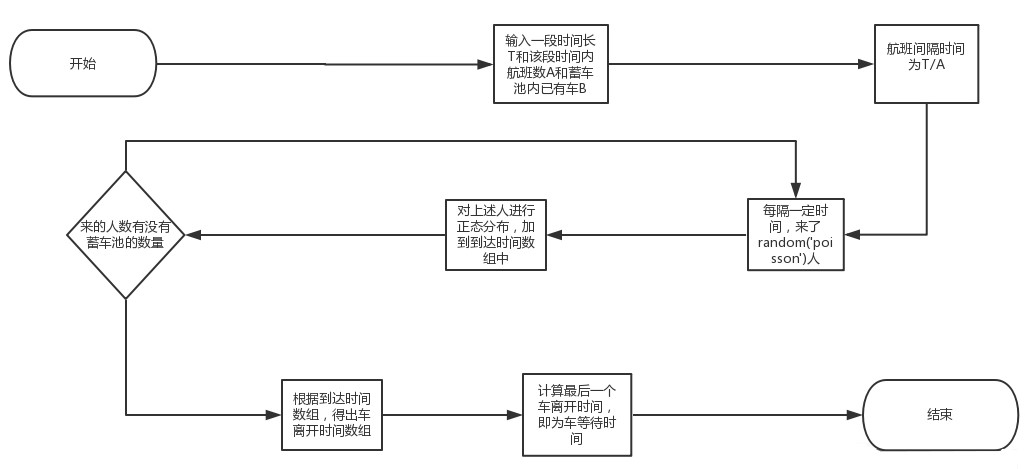
\includegraphics[width=0.8\textwidth]{img/program1.jpg}
	\caption{出租车等待时间模拟程序框图}
	\label{fi:program1}
\end{figure}
\par
该计算机程序的算法的运行主要分为如下几个步骤:
\begin{enumerate}[(1)]
	\item 程序接收输入的两个数据:一段时间内的航班数量\flightnum 和此时蓄车池内的出租车数量\taxinum ,由此计算出航班之间的间隔时间。
	\item 当每一架航班到达时,程序调用random函数根据泊松分布的规律,计算出每一架航班的人数。
	\item 将每一架航班到达的人数按照正态分布的时间规律,加入到不同时间段内的人数的数组中,实现排队队列的模拟功能。直到到达队列中的人数达到蓄车池内的出租车能够容纳的人数$N$为止,结束循环。
	\item 模拟一个队列,将各个时间的排队的数量依次加入乘车队列中,与此同时蓄车池内的出租车按照一定的时间间隔进行载客。最后计算整个过程花费的时间,并输出结果。
\end{enumerate}
通过运行如图所示的程序,我们得到了不同条件下的出租车司机需要等待的时长。取不同的\flightnum 和\taxinum 的值,输入程序,可以得到如图\ref{fi:problem1func}所示的函数图像。
\begin{figure}[H]
	\centering
	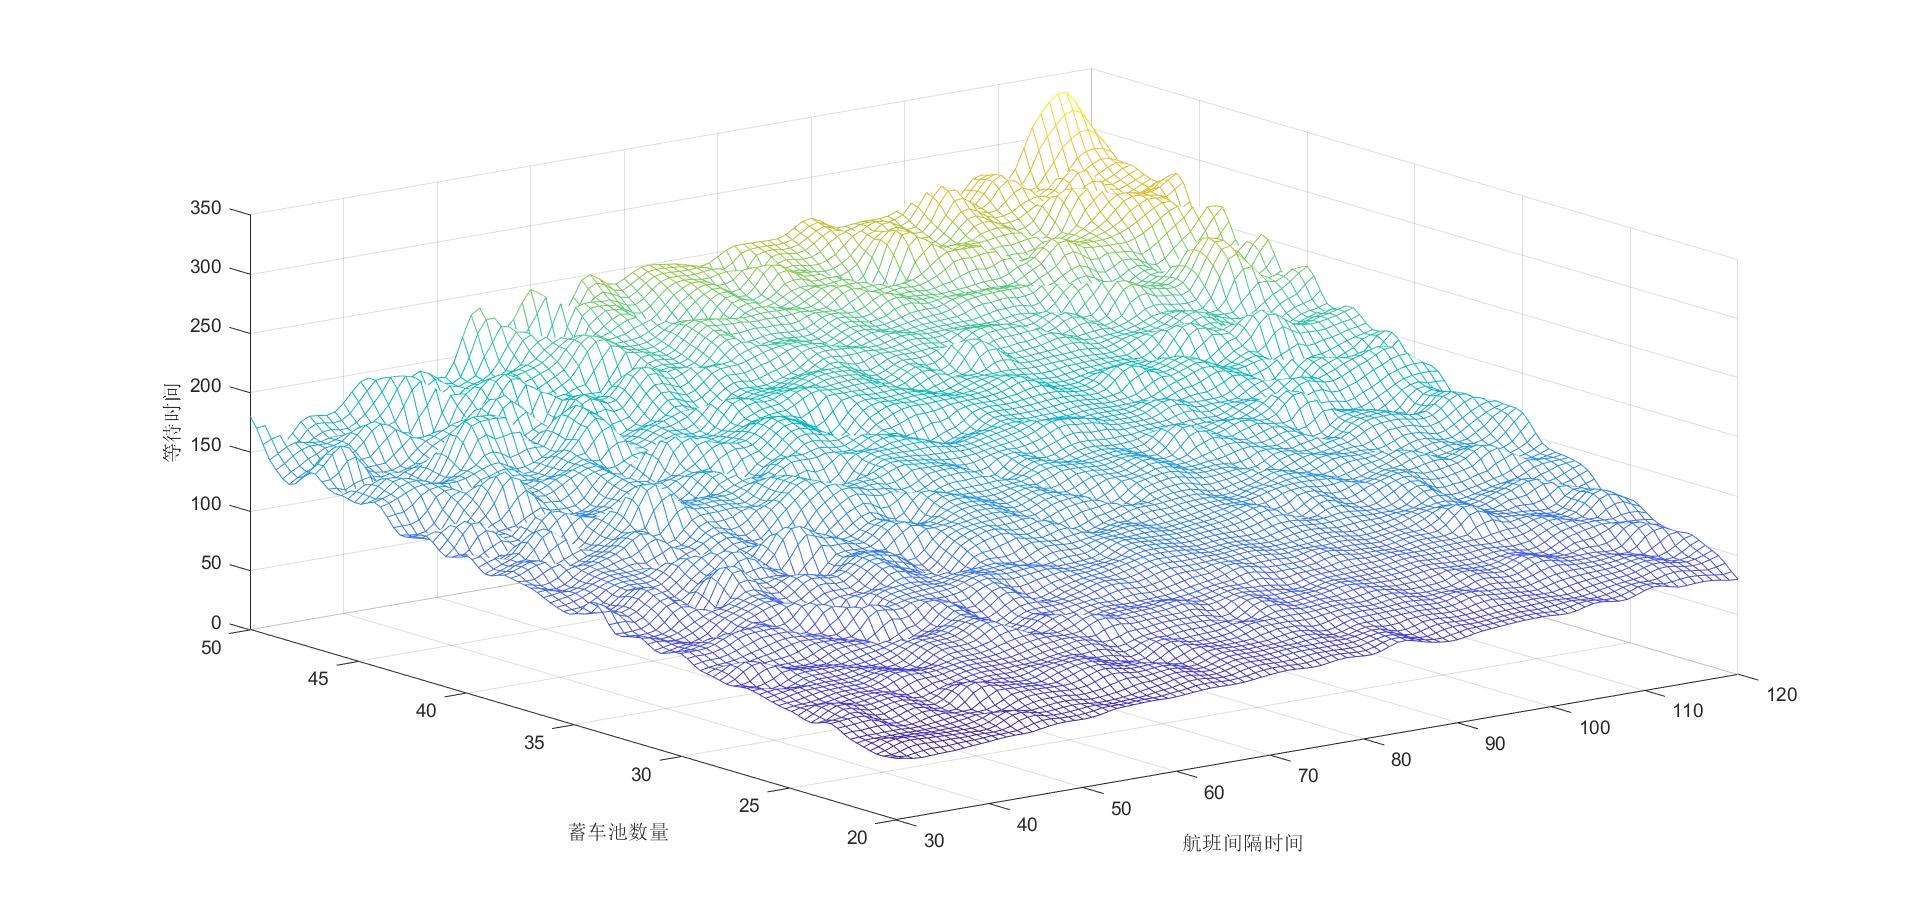
\includegraphics[width=1.0\textwidth]{img/problem1_func.jpg}
	\caption{\waittime$(\mbox{\flightnum,\taxinum})$函数图像}
	\label{fi:problem1func}
\end{figure}
\par
对于出租车收益,通过联立式\ref{eq:E1}、式\ref{eq:t2}和式\ref{eq:E2}可以得到等待时间\waittime 的分界值:
\begin{equation}
	\mbox{\waittime}_0=\frac{\overline{E_c}-\overline{E_{wo}}\cdot t_r}{\overline{E_t}-\overline{E_o}+\overline{E_{wo}}}
	\label{eq:tw}
\end{equation}
\par
综上所述,根据如下关系,可以得出出租车司机的最佳决策:
\begin{equation}
	\begin{cases}
		\mbox{  空载返回} &  \mbox{\waittime}(\mbox{\flightnum,\taxinum})\ge\mbox{\waittime}_0 ,\\
        \mbox{  等待载客} &  \mbox{\waittime}(\mbox{\flightnum,\taxinum})<\mbox{\waittime}_0  .
	\end{cases}
\end{equation}
\subsection{问题二的解答}
对于问题二,我们从各种渠道收集了关于国内某城市的机场和出租车的多种数据,用于对问题一中建立的模型进行正确性的分析与评估。\par
\begin{enumerate}[(1)]
	\item \textbf{出租车等待时间阈值计算。}\par
	我们收集了问题一中的模型中所需要的基本数据,这些数据在表中列出。
	\begin{table}[H]
		\centering
		\caption{城市出租车基本数据\cite{taxidata,taxireport}} 
		\label{table-symbol}
		\begin{tabular*}{0.31\textwidth}{ccc}
			\toprule
			项目 & 值 & 单位 \\
			\midrule
			平均车速 & 31.23 & $km/h$ \\
			空驶率 & $21.13\%$ & \\
			单价 & 1.82 & 元$/km$ \\
			油费 & 0.54 & 元$/km$ \\
			$\overline{E_c}$ & 62 & 元 \\
			$t_r$ & 50 & min \\
			\bottomrule
		\end{tabular*}
	\end{table}
	根据这个表格,可以计算出单位时间出租车平均收入$\overline{E_t}=0.75\mbox{元}/min$,单位时间出租车正常行驶平均油费$\overline{E_o}=0.28\mbox{元}/min$,排队中出租车单位时间平均油费$\overline{E_{wo}}=0.14\mbox{元}/min$。将该数据与上表数据代入式\ref{eq:tw}进行计算,计算得到的阈值:
	\begin{equation}
		\mbox{\waittime}_0=\frac{\overline{E_c}-\overline{E_{wo}}\cdot t_r}{\overline{E_t}-\overline{E_o}+\overline{E_{wo}}}=90\,min
	\end{equation}
	即若预计的等待时间$\hat{t_w}\ge90min$时,出租车选择空载返回;否则选择前往蓄车池内等待载客。
	\item \textbf{出租车等待时间预测。}\par
	根据某城市机场在一天内航班起降的数据,以及一天之内各个时间段的场内出租车数和出租车数据,使用问题一中的模型对出租车的等待时间进行了计算。其中,到达乘客乘坐出租车的占比为28\%,每架航班平均载客数量为100人\cite{taxidata,flightdata},取$\mu_1=10$,$\sigma=6$,得到如图\ref{fi:problem2func}所示的函数图像:
	\begin{figure}[H]
		\centering
		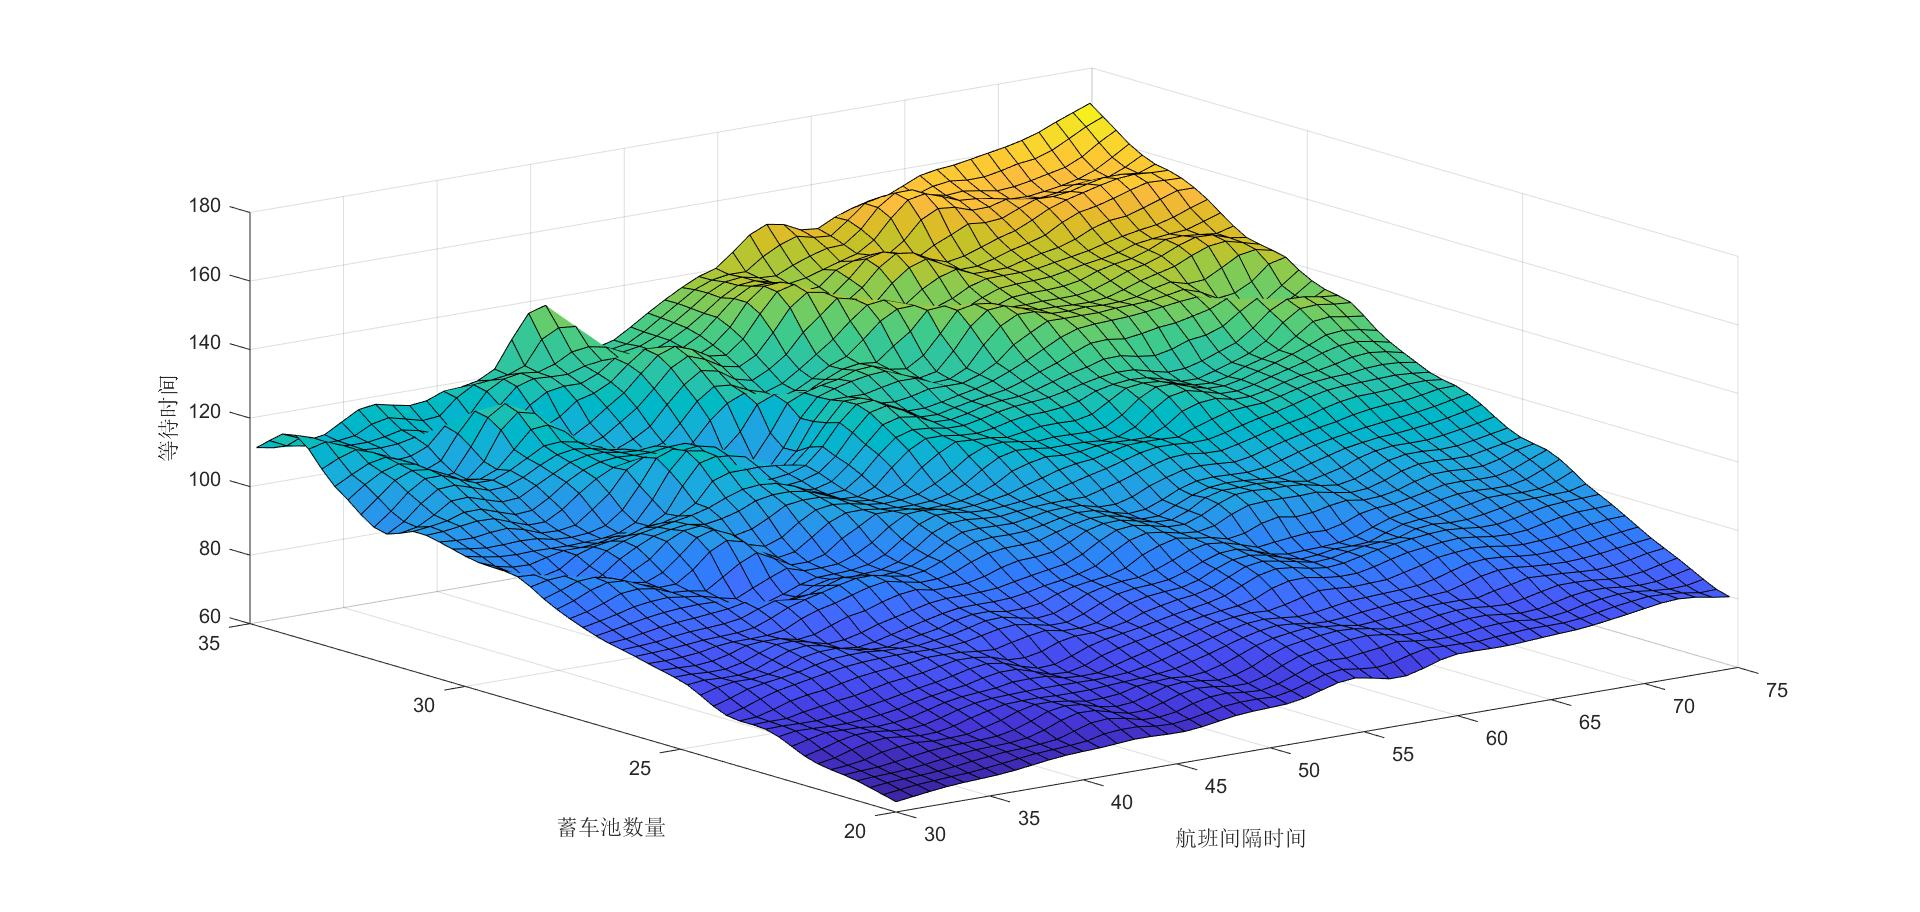
\includegraphics[width=0.8\textwidth]{img/problem2_func.jpg}
		\caption{实际参数下的\waittime$(\mbox{\flightnum,\taxinum})$函数图像}
		\label{fi:problem2func}
	\end{figure}
	\begin{figure}[H]   
		\centering   
		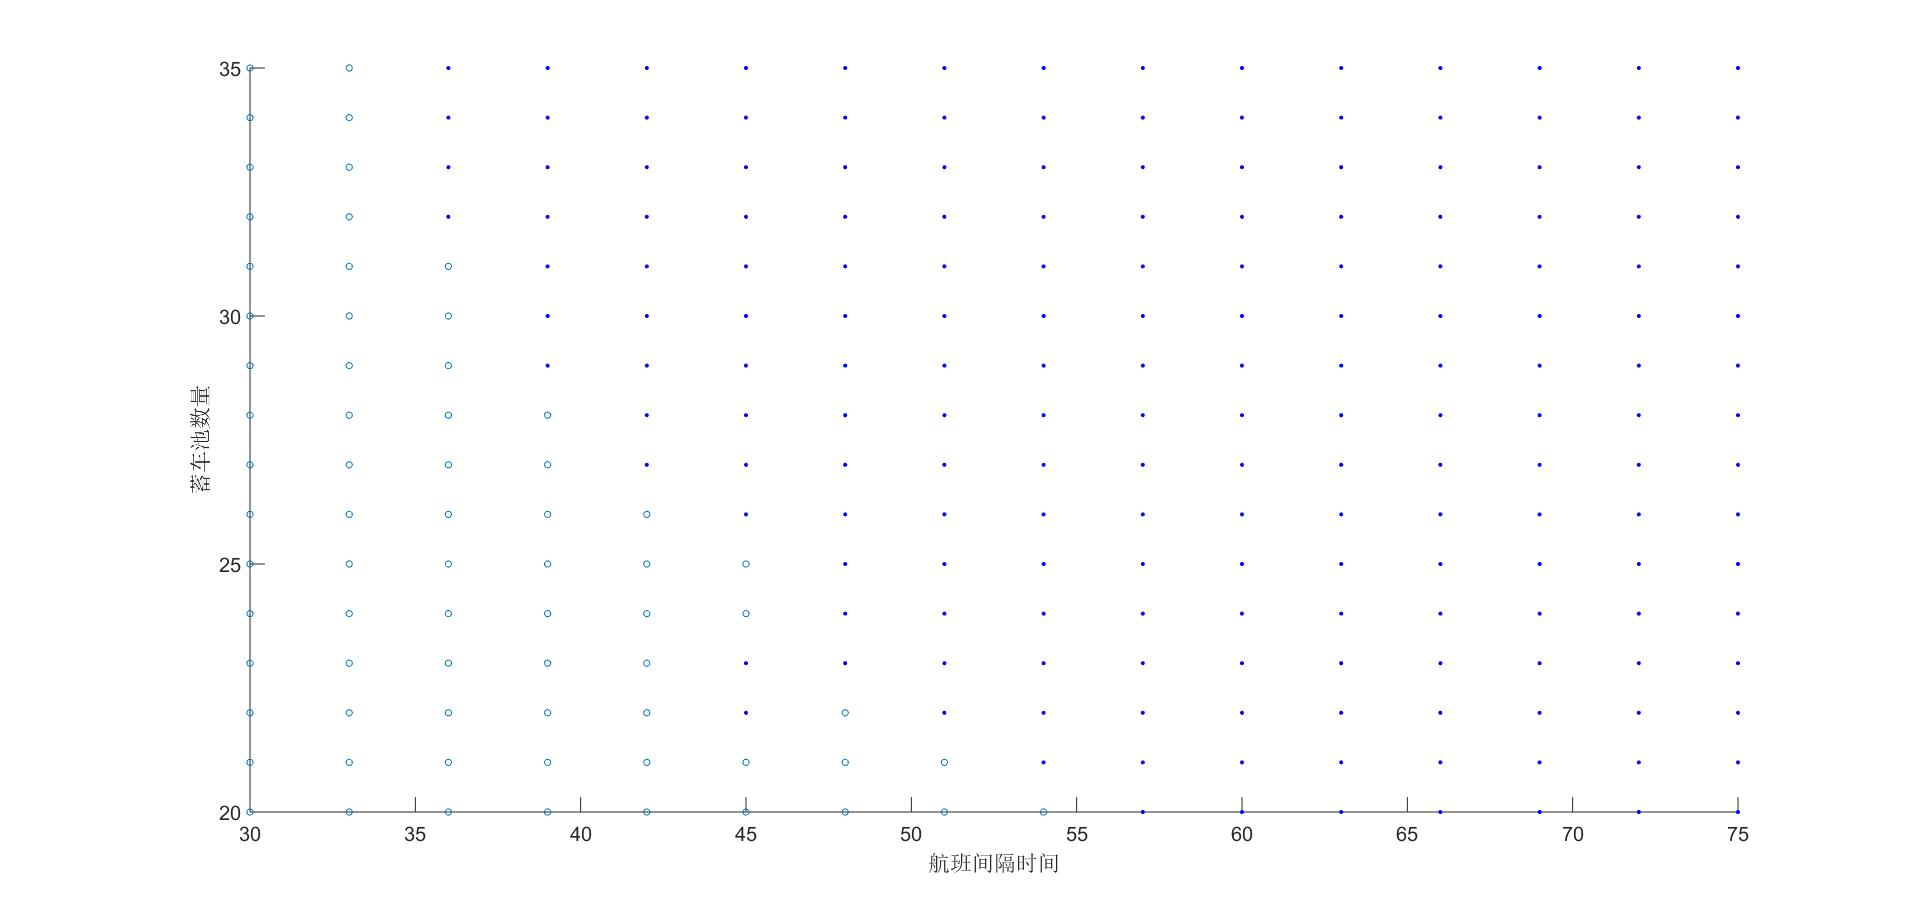
\includegraphics[width=1.0\textwidth]{img/problem2_pred.jpg}   
		\caption{出租车司机决策预测}   
		\label{fi:problem2pred}    
	\end{figure}
	图\ref{fi:problem2func}反映了在不同的\flightnum 和\taxinum 下的$\hat{t_w}$和$t_w$的大小分布情况,图\ref{fi:problem2pred}反应的是在不同的\flightnum 和\taxinum 下,出租车做出的决策的预测是空载返回(实心点)或是进入蓄车池等待载客(空心点)。\par
	根据预测得到的不同\flightnum 和\taxinum 下的$\hat{t_w}$与$t_w$进行比较,计算出模型的相对误差:
	\begin{equation}
		e_1=\frac{\left| \hat{t_w}-t_w\right| }{t_w}\times100\%=10.36\%
	\end{equation}
	由此可以看出,该模型与实际情况的误差在合理范围之内,可以用于预测现实情况下的司机的等待时间。	
\end{enumerate}
\subsection{问题三的解答}
本文建立了关于问题三的两种可能的模型:双车道停车模型和单车道停车模型,现在对两种模型代入特定的数据,求解模型的最优值。考虑到实际中航站楼现有的设施情况以及客流秩序安排的便捷性和合理性,我们在单停车道模型中取乘车点数目$C=2$,带入式\ref{eq:wq2}进行计算,并化简得到:
\begin{equation}
	W_{q2}=\frac{4\rho^3}{\lambda_2(1-\rho^2)}
\end{equation}
若实际情况中,单停车道模型相较于双车道停车模型更好,即:
\begin{equation}
	\frac{\lambda_2}{\mu_2(\mu_2-\lambda_2)}>\frac{4\rho^3}{\lambda_2(1-\rho^2)}
	\label{eq:wq1_wq2}
\end{equation}
解不等式\ref{eq:wq1_wq2},得:
\begin{equation}
	1<\frac{\lambda_2}{\mu_2}<2
\end{equation}
当$\frac{\lambda_2}{\mu_2}\ge2$时,由于两个模型的服务速度均小于顾客到访的速度,故队伍的长度不收敛,无法计算出此时的平均等待时间,此时需要采用例如限流等措施来控制人流量的大小。\par
根据国内某机场统计得到的数据平均值\cite{flightdata},我们可以得到如下表的参数值:
\begin{table}[H]
	\centering
	\caption{问题三模型的实际参数} 
	\label{table-symbol}
	\begin{tabular*}{0.31\textwidth}{p{3.5cm}p{2cm}}
		\toprule
		项目 & 值 \\
		\midrule
		$\mu_2$ & 9.375 \\
		$\lambda_2$ & 17.68 \\
		$\lambda_2/\mu_2$ & 1.86 \\
		\bottomrule
	\end{tabular*}
\end{table}
由此可知,根据此机场该时间段的实际数据,使用单车道停车模型($C=2$)更为合适。综上所述,在模型定义的范围内$(0<\frac{\lambda_2}{\mu_2}<2)$,我们可以得到如下的选择方案与人流量、车流量的关系:
\begin{equation}
	\begin{cases}
		\mbox{  双车道停车模型}\quad & 0<\frac{\lambda_2}{\mu_2}\le1 \\
		\mbox{  单车道停车模型}(C=2)\quad & 1<\frac{\lambda_2}{\mu_2}<2 \\
	\end{cases}
\end{equation}
\subsection{问题四的解答}
根据上述的算法,我们设计了如下伪代码的算法来模拟这个过程,计算出出租车单位时间的方差平均值$\overline{E_a}$。
\renewcommand{\algorithmicrequire}{\textbf{Input:}} 
\renewcommand{\algorithmicensure}{\textbf{Output:}}
\begin{algorithm} [H] 
	\caption{模拟机场出租车算法} %算法的题目 
	\label{al:problem4} %算法的标签 
	\begin{algorithmic}[1] %此处的[1]控制一下算法中的每句前面都有标号 
		\REQUIRE {参数$\alpha$、$\beta$和阈值$r_0$}
		\ENSURE{出租车的单位时间平均收入的方差$\sigma^2$}
		\WHILE{剩余的出租车数量$\ge 0$}
		\IF{下一辆出租车的优先级为高}
		\STATE 加入优先车道
		\ELSE
		\STATE 加入普通车道
		\ENDIF
		\STATE 按照$\beta:1$比例从车道内选出一辆车
		\STATE $d\leftarrow N(\mu,\sigma^2)$
		\IF{$d>d_0\;\mathbf{and}\;choose=True$}
		\STATE $r\leftarrow f(d,t_w)$
		\IF{$r\le r_0$}
		\STATE 优先级为高
		\ELSE
		\STATE 优先级为低
		\ENDIF
		\ELSE
		\STATE $\overline{E_{ai}}\leftarrow \frac{1}{T_{total}}\sum\limits_j E_j(d)$
		\ENDIF
		\ENDWHILE
		\STATE $\sigma^2\leftarrow var(\overline{E_a})$
	\end{algorithmic} 
\end{algorithm}
使用该算法,可以求得在不同参数条件下的方差$\sigma^2$,要调整参数使方差最小化,可以使用如下的几种全局优化算法来快速求得条件范围内的最小值。
\begin{enumerate}[(1)]
	\item \textbf{遗传算法。}\par
	遗传算法(Genetic Algorithms,\;GA)代表了一种用于了解多个参数关于模型的结果的相关因素的方法,而任何东西都可以用作遗传算法的数据。包括数字、文字、图像等。在遗传算法的进化计算的过程中,模拟生物的基因变异或交换的过程,允许那些适应度高的的基因进一步繁殖,适应度低的基因则死亡\cite{ga_al}。\par
	通过遗传算法,我们可以很轻松地计算出多参数的连续函数在指定范围内的最优解。我们构建了如下的有限范围内的优化问题,用于遗传算法的计算:
	\begin{equation}
		\begin{aligned}
			\min\quad & \sigma^2(\overline{E_a}) \\
			s.t.\quad & 1\le \alpha \le 100 \\
			& 1000\le r_0 \le 10000 \\
			& 1\le \beta \le 10 \\
		\end{aligned}
	\end{equation}
	设定其它参数(详见附录中程序数据)后,另外将上述范围输入遗传算法运行,最终计算的方差的最小值:$\sigma_{min}^2=0.0272$,此时$\alpha=99.8,r_0=2421.8,\beta=2.8$。
	\item \textbf{模拟退火算法。}\par
	模拟退火算法(Simulated Annealing, SA)是一种局部搜索算法的扩展。它模拟了金属在退火过程中的能量变化,在每一次迭代的过程中以一定的机率选择相邻区域能量较大的状态\cite{sa_al}。它从理论上而言是一种全局最优算法,能够快捷地找到一个多元函数的全局最小值或最大值点。\par
	设定如遗传算法中的参数和数据范围,输入模拟退火算法进行计算,最终计算的方差的最小值:$\sigma_{min}^2=0.0281$,此时$\alpha=99.9,r_0=4898.1,\beta=9.2$。
	\item \textbf{粒子群算法。}\par
	粒子群优化算法(Particle Swarm optimization,\;PSO)是通过模拟鸟群的觅食行为,形成的一种基于群体协作原理的随机搜索算法。在PSO算法中,所有的粒子都有一个适应值和速度,通过不断迭代,跟踪个体极值和全局极值,来找到全局的最优解\cite{pso_al}。\par
	设定如遗传算法中的参数和数据范围,输入粒子群算法进行计算,最终计算的方差的最小值:$\sigma_{min}^2=0.0271$,此时$\alpha=100.0,r_0=2420.8,\beta=1.0$。
\end{enumerate}
\begin{figure}[H]
	\centering
	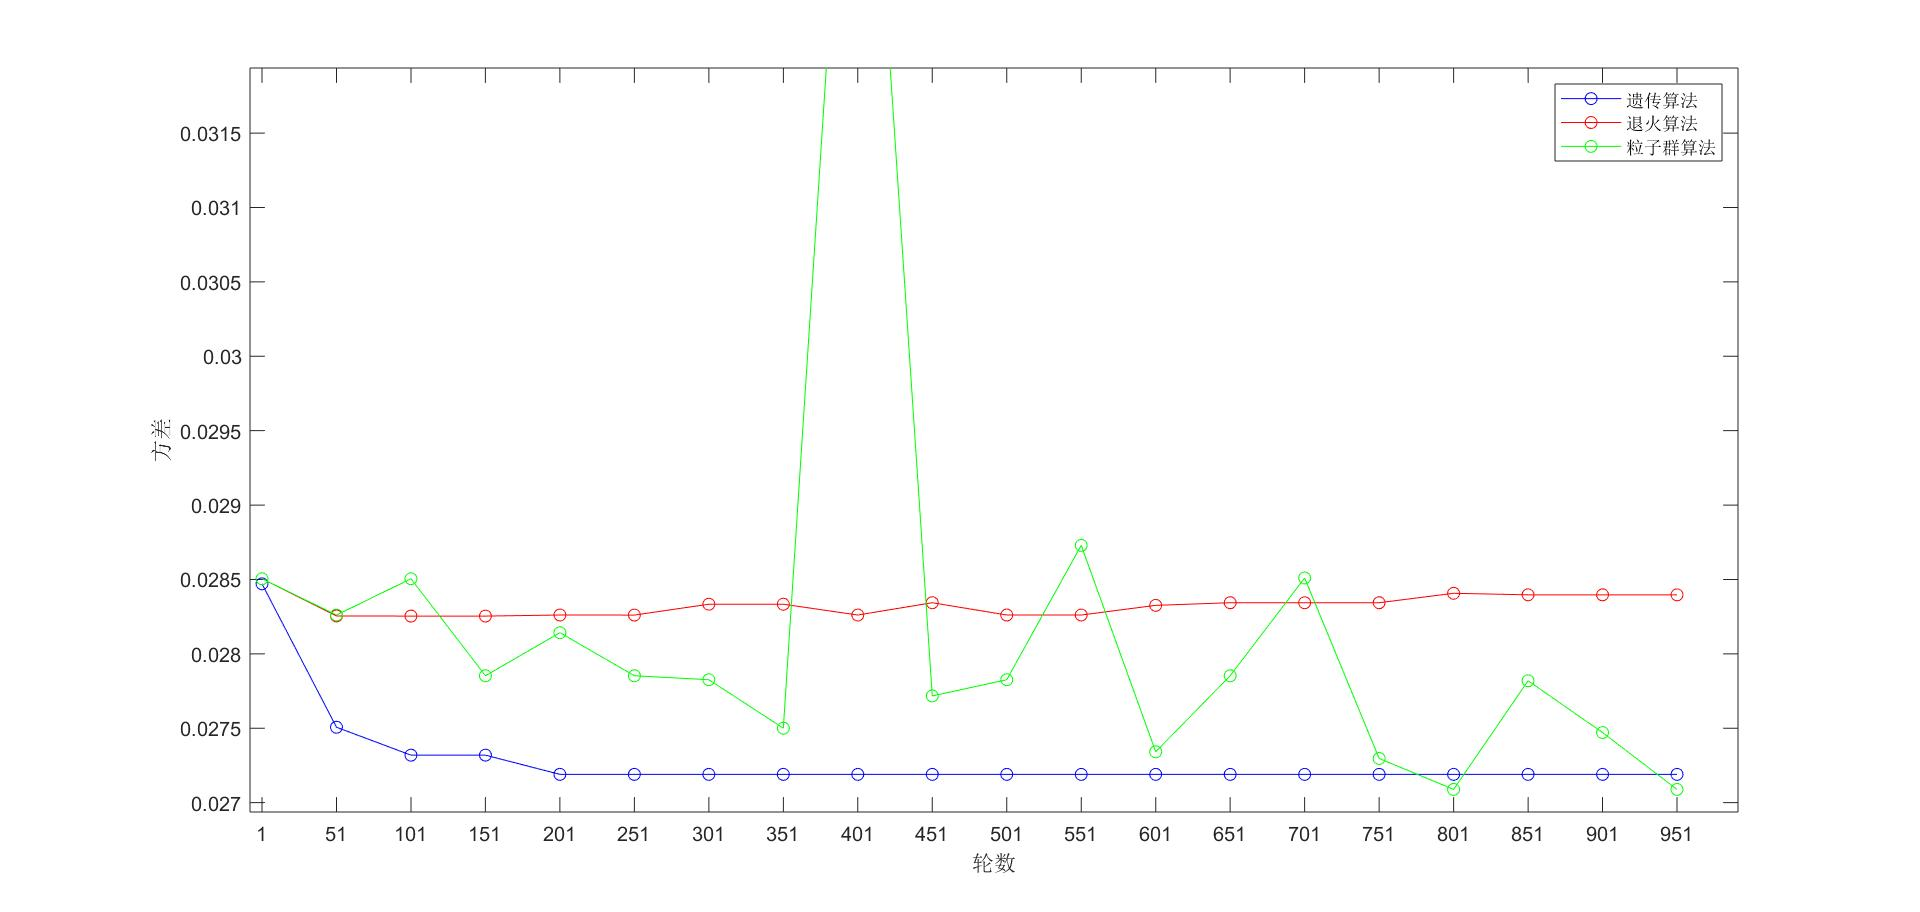
\includegraphics[width=1.0\textwidth]{img/problem4_al.jpg}
	\caption{三种优化算法的比较}
	\label{fi:problem4al}
\end{figure}
\par
图为以上三种算法收敛的过程,通过比较以上三种全局优化算法,可以看出粒子群算法对本模型最为适用。收敛速度快,且得到的方差结果最小。\par
综上所述,对于本模型假定的其余参数,当模型的三个主要参数为$\sigma_{min}^2=0.0271,\alpha=100.0,r_0=2420.8,\beta=1.0$时,出租车司机的收益最为均衡。
\section{模型总结}
\subsection{灵敏度分析}
我们对出租车司机决策模型做出分析。对于不同的机场,其蓄车池的容量可能有较大的差距,而即使是对同一座机场,不同的时间也会有不同的航班到达间隔。而考虑到出租车司机在获取这两个信息时都可能存在一定的偏差,因此,有必要对该模型对蓄车池的容量和航班到达间隔的变化的灵敏度做出分析。\par
\begin{figure}[H]
	\begin{minipage}[t]{0.5\linewidth}   
	  \centering   
	  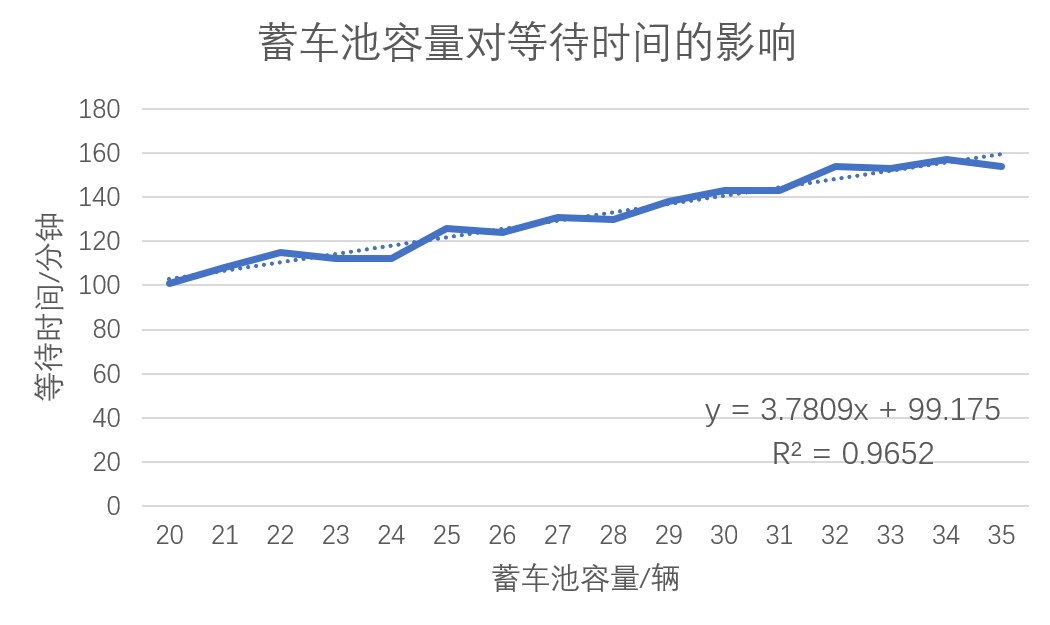
\includegraphics[width=\textwidth]{img/check_1.jpg}   
	  \caption{蓄车池容量对等待时间的影响}   
	  \label{fi:check_1}   
	\end{minipage}
	 \begin{minipage}[t]{0.5\linewidth}
		\centering   
		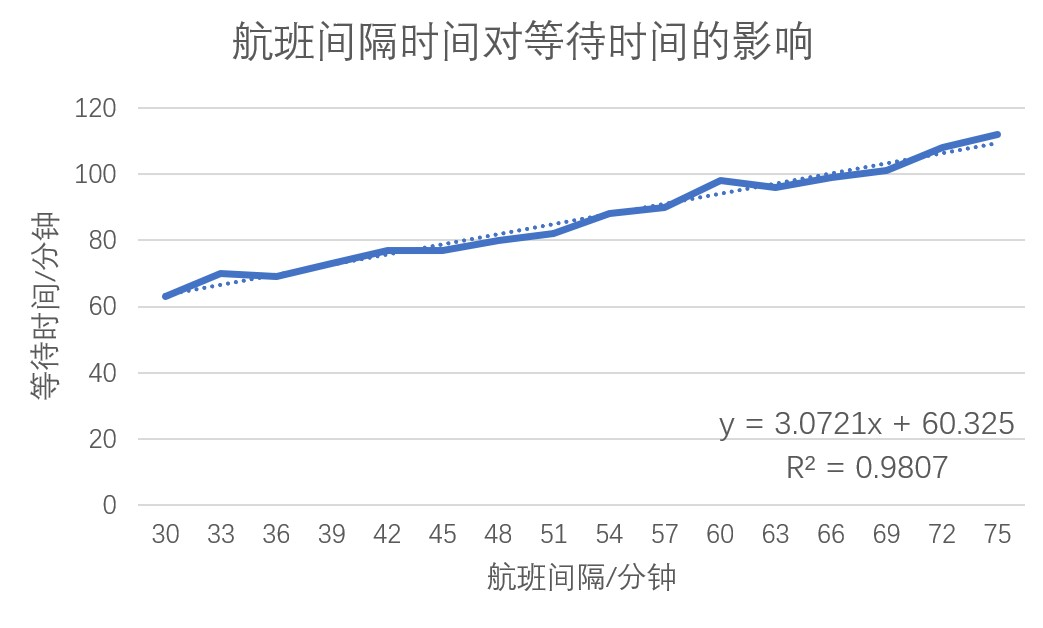
\includegraphics[width=\textwidth]{img/check_2.jpg}   
		\caption{航班间隔时间对等待时间的影响}   
		\label{fi:check_2}   
	  \end{minipage} 
  \end{figure}
从模型计算得出的数据和图\ref{fi:check_1}、图\ref{fi:check_2}容易看出,蓄车池容量的变化对等待时间的影响,比航班间隔变化对等待时间的影响更大。也即等待时间对蓄车池的容量更加敏感。因此对于司机来说,正确的判断蓄车池内此时正在等候的汽车数目,更加有利于其做出正确的判断。这也与实际情况符合较好:一般的停车场都会用电子显示屏显示出此时停车场内的容量,而航班到达间隔这个信息要稍加难获取一些。
\subsection{模型优点}
\begin{enumerate}
	\item 模型在建立时经历了较为广泛的调研,考虑了很多不同的实际情况,在设置不同的参量时使用了大量来源于实际生活的数据,增强了模型的普适性以及实际意义。
	\item 在建立模型时,我们使用了计算机编程的方法,对每个模型的过程都进行了仿真,将预测得到的数据和实际数据进行了对比并将对比结果进行了可视化表示,提高了结果的准确度,也使得结果更加直观。
	\item 在解决问题二的时候,我们采用了网络爬虫技术收集了一座机场的数据,得到了大量真实且精确的数据,也避免了把人力无谓地浪费在实地收集数据上。
	\item 在解决问题四时,我们采用了遗传算法来对模型中的参数进行优化,使参数的选择更加合理。
\end{enumerate}
\subsection{模型缺点}
\begin{enumerate}
	\item 由于本题涉及到的实际情景非常复杂,可能影响结果的变量有很多,我们选择性地忽略了其中一些对结果影响不大的变量作为近似,比如问题三中隧道和车辆的长度等问题。
	\item 由于模型考虑了较多的实际情况,导致有些过程略显繁琐。
\end{enumerate}

\newpage
\bibliography{ref}

\newpage
\appendix
\textbf{附录}
\section{模型代码}
\subsection{出租车等待时间计算代码}
\begin{lstlisting}
	%% 设置导入选项
opts = spreadsheetImportOptions("NumVariables", 5);

% 指定工作表和范围
opts.Sheet = "data";
opts.DataRange = "A2:E1232";

% 指定列名称和类型
opts.VariableNames = ["VarName1", "VarName2", "VarName3", "VarName4", "VarName5"];
opts.SelectedVariableNames = ["VarName1", "VarName2", "VarName3", "VarName4", "VarName5"];
opts.VariableTypes = ["categorical", "double", "double", "double", "double"];
opts = setvaropts(opts, 1, "EmptyFieldRule", "auto");

% 导入数据
tbl = readtable("data.xlsx", opts, "UseExcel", false);

%% 转换为输出类型
VarName1 = tbl.VarName1;
VarName2 = tbl.VarName2;
VarName3 = tbl.VarName3;
VarName4 = tbl.VarName4;
VarName5 = tbl.VarName5;

%% 清除临时变量
clear opts tbl


%% 设置导入选项
opts = spreadsheetImportOptions("NumVariables", 3);

% 指定工作表和范围
opts.Sheet = "Sheet1";
opts.DataRange = "A1:C242";

% 指定列名称和类型
opts.VariableNames = ["VarName1", "VarName2", "VarName3"];
opts.SelectedVariableNames = ["VarName1", "VarName2", "VarName3"];
opts.VariableTypes = ["double", "double", "double"];

% 导入数据
data2 = readtable("data2.xlsx", opts, "UseExcel", false);

%% 转化为输出类型
VarName6=data2.VarName1;
VarName7=data2.VarName2;
VarName8=data2.VarName3;
%% 清除临时变量
clear opts


%% 导入每分钟的航班
flights=zeros(1440,1);
for i=2:242
    if VarName6(i,1)>=18&&VarName6(i,1)<=23
        tt=(VarName6(i,1)-18)*60+VarName7(i,1);
    else
        tt=(6+VarName6(i,1))*60+VarName7(i,1);
    end
    if tt~=0
        flights(tt,1)=flights(tt,1)+1;
    end
end
        
%% 生成等待时间模型
x1=30:3:75;
y1=20:1:35;
z1=zeros(16,16);
x2=[]; x3=[]; y2=[]; y3=[];
ii=1;
for i=x1
    jj=0;
    for j=y1
        total=0;
        jj=jj+1;
        for k=1:20
            total=total+waittime(1,i,j);
        end
        z1(ii,jj)=floor(total/20);
        %if floor(total/20)>=90
        %   x2=[x2,i];
        %    y2=[y2,j];
        %else
        %   x3=[x3,i];
        %    y3=[y3,j];
        %end
    end
    ii=ii+1;
end
figure
xx=linspace(30,120,100);
yy=linspace(20,50,100);
zz=griddata(x1,y1,z1,xx,yy','cubic');
surf(xx,yy,zz);
xlabel('航班间隔时间');
ylabel('蓄车池数量');
zlabel('等待时间');



%% 生成误差模型
wucha=zeros(1231,1);
wucha2=zeros(1231,1);
lilun=zeros(1231,1);
shiji=zeros(1231,1);
%x1=[]; x2=[]; y1=[]; y2=[];
for i=1:1000
    num=0;
    for j=i:i+120
        if flights(j,1)~=0
            num=num+1;
        end
    end
    if num==0
        continue;
    end
    tmp=waittime(num,120,VarName3(i,1));
    tmp2=i;
    ww=0;
    numofleave=0;
    while numofleave<=VarName3(i,1)&&VarName5(tmp2+30,1)<=VarName3(i,1)-numofleave
        tmp2=tmp2+30;
        ww=ww+30;
        numofleave=numofleave+VarName5(tmp2,1);
    end
    if VarName5(tmp2+30,1)>VarName3(i,1)-numofleave
        ww=ww+(VarName3(i,1)-numofleave)/VarName5(tmp2+30,1)*30;
    end
    ww=round(ww);
    if ww>=90
        x1=[x1,floor(120/num)];
        y1=[y1,VarName3(i,1)];
    else
        x2=[x2,floor(120/num)];
        y2=[y2,VarName3(i,1)];
    end
    wucha(i,1)=(tmp-ww);
    wucha2(i,1)=abs(tmp-ww)/ww;
    lilun(i,1)=tmp;
    shiji(i,1)=ww;
end
x1=x1(1:200);
y1=y1(1:200);
x2=x2(1:200);
y2=y2(1:200);
anss=wucha2(1:130,:);
xd=mean(anss);
\end{lstlisting}
\subsection{出租车等待时间计算代码子函数}
\begin{lstlisting}
	function f = waittime(inputArg1,inputArg2,inputArg3)
N=inputArg1;     %未来一段时间内来的航班数
T=inputArg2;     %未来一段时间的持续时间minutes
A=floor(T/N);    %minutes;航班每隔多少时间来一趟
B=inputArg3;     %蓄车池个数
t0=1;            %每个人上车需要1minutes
delta=25;        %每来一个航班人走到出租车点的平均时间
t=0;             %time 
C=28;            %航班人数来乘车的平均数
sigma=6;         %方差
arrive=zeros(1000,1);
leave=zeros(1000,1);
currentnum=0;  
while currentnum<=B
    t=t+1;
    if(mod(t,A)==0)
        n=random('poisson',C);
        currentnum=currentnum+n;
    else
        n=0;
    end
    for i=1:n
        time=floor(normrnd(t+delta,sigma));
        while time<t
            time=floor(normrnd(t+delta,sigma));
        end
        arrive(time,1)=arrive(time,1)+1;
    end
end
currentnum=0;
t=0;
while 1
    t=t+1;
    if arrive(t,1)~=0
        break;
    end
end
i=t;
while currentnum<=B
   if arrive(i,1)~=0
       if arrive(i,1)<=4
           num=round(rand()*arrive(i,1));
           while num==0
               num=round(rand()*arrive(i,1));
           end
       else
           num=round(rand()*4);
           while num==0
           num=round(rand()*4);
           end
       end
       arrive(i,1)=arrive(i,1)-num;
       currentnum=currentnum+num;
       if i<t
           leave(t+t0,1)=leave(t+t0,1)+num;
           t=t+t0;
       else
           leave(i+t0,1)=leave(i+t0,1)+num;
           t=i+t0;
       end
   else
       i=i+1;
   end
end
   f=t;
end


\end{lstlisting}
\subsection{出租车费用计算代码}
\begin{lstlisting}
	function f = fee(distance)
distance=distance/1000;
if distance<=3
    f=14;
else
    if distance<=15
        f=14+(distance-3)*2.5;
    else
        f=14+30+(distance-15)*3.6;
    end
end
end

\end{lstlisting}
\subsection{计算优先权的函数}
\begin{lstlisting}
	function f = fun1(waitime,shouyi,afa)
if shouyi==0
    f=-waitime;
else
    f= -waitime+shouyi*afa;
end
end
\end{lstlisting}
\subsection{模拟基于优先权出租车调度代码}
\begin{lstlisting}
	function fangcha=thepath(x)
global oo;
global resukts;
afa=x(1);
r0=x(2);
bili=x(3);
oo=oo+1;
%% 设置导入选项
opts = spreadsheetImportOptions("NumVariables", 2);

% 指定工作表和范围
opts.Sheet = "Sheet1";
opts.DataRange = "A2:B5000";

% 指定列名称和类型
opts.VariableNames = ["VarName1", "VarName2"];
opts.SelectedVariableNames = ["VarName1", "VarName2"];
opts.VariableTypes = ["double", "double"];

% 导入数据
tbl = readtable("suijibiao.xlsx", opts, "UseExcel", false);

%% 转换为输出类型
suijishu1 = tbl.VarName1;
suijishu2 = tbl.VarName2;

%% 清除临时变量
clear opts tbl


%%
allnum=500;   %汽车总数
v=250;        %平均车速30km/h 250m/min
youfei=0.7;  %油费
fenjie=10000;   %分界线 长短距离 训练 m
s1=1:allnum;   %车排队序列 低优先级 下标代表目前所在位 数值代表车的标号
s2=[];         %高优先级
waitime=zeros(allnum,1);  %车目前等待时间 下标代表车编号
avevas([1:allnum],1)=aveva; %车目前平均收益 下标代表车标号
leave=0;            %不会再回来车的数量
curnum=0 ;  %目前被超车的次数
times=zeros(allnum,1);  %时间事件表 若值不为0,即为该时刻有车来排队
allwaittime=zeros(allnum,1); %每一辆车 总等待时间
alldistance=zeros(allnum,1); %每一辆车 总路程
results=zeros(allnum,1);  %结果 最后的总收益
t=0;        %计时
backto=zeros(allnum,1);  %回来的次数
sigma=3000;   %标准差
mu=10000;     %平均值
MAX=9999;
zz=1;
zzz=1;
while leave<allnum
    t=t+1;  %时间加1
    
    % 所有正在等待车时间加一
    for i=s1
        if i~=0
            waitime(i,1)=waitime(i,1)+1;
            allwaittime(i,1)=allwaittime(i,1)+1;
        end
    end
    for i=s2
        if i~=0
            waitime(i,1)=waitime(i,1)+1;
            allwaittime(i,1)=allwaittime(i,1)+1;
        end
    end
    
    % 将返程车加入排队队列中
    for j=1:allnum
        if times(j,1)==t  %j为返程的车
            if fun1(waitime(j,1),results(j,1),afa)<r0
                s2=[s2,j];
                backto(j,1)=fun1(waitime(j,1),results(j,1),afa);
            else
                s1=[s1,j];
                backto(j,1)=fun1(waitime(j,1),results(j,1),afa);
            end
            waitime(j,1)=0;
            
        end
    end
    
    if length(s1)+length(s2)==0
        continue;
    end
    
    % 从排队序列选出下一次走的车
    if ~isempty(s2)&&(curnum<bili||isempty(s1))
        curno=s2(1,1);
        curnum=curnum+1;
        if length(s2)>1
            s2=s2(2:end);
        else
            s2=[];
        end
    else
        curno=s1(1,1);
        curnum=0;
        if length(s1)>1
            s1=s1(2:end);
        else
            s1=[];
        end
    end
   
    % 获得随机路程
    tmp=suijishu1(zz);
    zz=zz+1;
    while tmp<=0
        tmp=suijishu1(zz);
        zz=zz+1;
    end
    if tmp>=fenjie
        results(curno,1)=results(curno,1)+fee(tmp)-tmp/1000*youfei;
        alldistance(curno,1)=alldistance(curno,1)+tmp;
        leave=leave+1;
    else
        results(curno,1)=results(curno,1)+fee(tmp)-tmp/1000*youfei;
        alldistance(curno,1)=alldistance(curno,1)+tmp;
        therand=suijishu2(zzz);
        zzz=zzz+1;
        if therand>=0.5
            results(curno,1)=results(curno,1)-tmp/1000*youfei;
            alldistance(curno,1)=alldistance(curno,1)+tmp;
            times(curno)=round(t+tmp/v*2);
        else
            leave=leave+1;
        end
    end
end

for i=1:allnum
    allwaittime(i,1)=allwaittime(i,1)-i+1;
    avevas(i,1)=results(i,1)/(allwaittime(i,1)+alldistance(i,1)/v);
end
fangcha=var(avevas);
resukts(oo,1)=fangcha;
end
\end{lstlisting}
\end{document}